%%
%% This is file `sample-sigconf.tex',
%% generated with the docstrip utility.
%%
%% The original source files were:
%%
%% samples.dtx  (with options: `sigconf')
%% 
%% IMPORTANT NOTICE:
%% 
%% For the copyright see the source file.
%% 
%% Any modified versions of this file must be renamed
%% with new filenames distinct from sample-sigconf.tex.
%% 
%% For distribution of the original source see the terms
%% for copying and modification in the file samples.dtx.
%% 
%% This generated file may be distributed as long as the
%% original source files, as listed above, are part of the
%% same distribution. (The sources need not necessarily be
%% in the same archive or directory.)
%%
%%
%% Commands for TeXCount
%TC:macro \cite [option:text,text]
%TC:macro \citep [option:text,text]
%TC:macro \citet [option:text,text]
%TC:envir table 0 1
%TC:envir table* 0 1
%TC:envir tabular [ignore] word
%TC:envir displaymath 0 word
%TC:envir math 0 word
%TC:envir comment 0 0
%%
%%
%% The first command in your LaTeX source must be the \documentclass command.
\documentclass[sigconf]{acmart}
\usepackage{balance} % For balanced columns on the last page
\usepackage[binary-units]{siunitx}
\usepackage{listings}

\sisetup{separate-uncertainty=true}

% Visible TODO notes
\newcommand{\todo}[1]{\textbf{\textsc{\textcolor{red}{(TODO: #1)}}}}

% Code colouring
\definecolor{NavyBlue}{rgb}{0.0,0.0,0.5}
\definecolor{OliveGreen}{rgb}{0.5,0.5,0.0}
\definecolor{Mulberry}{rgb}{0.77,0.29,0.55}
\definecolor{Maroon}{rgb}{0.5,0.0,0.0}
\lstset{language=Python,morekeywords={True,False},showstringspaces=false,basicstyle=\small\ttfamily\bfseries,keywordstyle=\color{Mulberry}\bfseries,identifierstyle=\color{NavyBlue}\bfseries,stringstyle=\ttfamily\color{OliveGreen}\bfseries,commentstyle=\ttfamily\color{Maroon}\bfseries,frame=none,upquote=true,morekeywords={True,False}}


%%
%% \BibTeX command to typeset BibTeX logo in the docs
\AtBeginDocument{%
  \providecommand\BibTeX{{%
    \normalfont B\kern-0.5em{\scshape i\kern-0.25em b}\kern-0.8em\TeX}}}

%% Rights management information.  This information is sent to you
%% when you complete the rights form.  These commands have SAMPLE
%% values in them; it is your responsibility as an author to replace
%% the commands and values with those provided to you when you
%% complete the rights form.
\copyrightyear{2022}
\acmYear{2022}
\setcopyright{rightsretained}
\acmConference[NICE 2023]{Neuro-Inspired Computational Elements Conference}{April 11-April 14, 2023}{San Antonio, USA}
\acmBooktitle{Neuro-Inspired Computational Elements Conference (NICE 2023), April 11-April 14, 2023, San Antonio, USA}
\acmDOI{XXXXXXX.XXXXXXX}
\acmISBN{978-1-4503-XXXX-X/18/06}


%%
%% Submission ID.
%% Use this when submitting an article to a sponsored event. You'll
%% receive a unique submission ID from the organizers
%% of the event, and this ID should be used as the parameter to this command.
%%\acmSubmissionID{123-A56-BU3}

%%
%% The majority of ACM publications use numbered citations and
%% references.  The command \citestyle{authoryear} switches to the
%% "author year" style.
%%
%% If you are preparing content for an event
%% sponsored by ACM SIGGRAPH, you must use the "author year" style of
%% citations and references.
%% Uncommenting
%% the next command will enable that style.
%%\citestyle{acmauthoryear}

%%
%% end of the preamble, start of the body of the document source.
\begin{document}

%%maintanance
%% The "title" command has an optional parameter,
%% allowing the author to define a "short title" to be used in page headers.
\title{Easy and efficient spike-based Machine Learning with mlGeNN}

%%
%% The "author" command and its associated commands are used to define
%% the authors and their affiliations.
%% Of note is the shared affiliation of the first two authors, and the
%% "authornote" and "authornotemark" commands
%% used to denote shared contribution to the research.
\author{James C Knight}
\email{J.C.Knight@sussex.ac.uk}
\orcid{0000-0003-0577-0074}
\affiliation{%
  \institution{University of Sussex}
  \department{School of Engineering and Informatics}
  \city{Brighton}
  \country{United Kingdom}
}

\author{Thomas Nowotny}
\email{T.Nowotny@sussex.ac.uk}
\orcid{0000-0002-4451-915X}
\affiliation{%
  \institution{University of Sussex}
  \department{School of Engineering and Informatics}
  \city{Brighton}
  \country{United Kingdom}
}
%%
%% By default, the full list of authors will be used in the page
%% headers. Often, this list is too long, and will overlap
%% other information printed in the page headers. This command allows
%% the author to define a more concise list
%% of authors' names for this purpose.
\renewcommand{\shortauthors}{Knight and Nowotny}

%%
%% The abstract is a short summary of the work to be presented in the
%% article.
\begin{abstract}
  Intuitive and easy to use application programming interfaces such as Keras have contributed majorly to the rapid acceleration of machine learning with artificial neural networks. Building on our recent work on translating ANNs to SNNs, we here present the mlGeNN interface as an easy way to define, train and test spiking neural networks on our efficient GPU based GeNN framework. We illustrate the use of mlGeNN by investigating the performance of a number of shallow spiking neural networks trained with the e-prop learning rule to recognise hand gestures from the DVS gesture dataset. We find that not only is mlGeNN vastly more convenient to use than the lower level PyGeNN interface, the new freedom to effortlessly and rapidly prototype different network architectures also gave us an unprecendent overview over how e-prop compares to other recently published results on the DVS gesture dataset across architectural details. 
\end{abstract}

%%
%% The code below is generated by the tool at http://dl.acm.org/ccs.cfm.
%% Please copy and paste the code instead of the example below.
%%
\begin{CCSXML}
<ccs2012>
   <concept>
       <concept_id>10010147.10010257.10010293.10011809</concept_id>
       <concept_desc>Computing methodologies~Bio-inspired approaches</concept_desc>
       <concept_significance>300</concept_significance>
       </concept>
   <concept>
       <concept_id>10010147.10010257.10010258.10010259</concept_id>
       <concept_desc>Computing meis thodologies~Supervised learning</concept_desc>
       <concept_significance>300</concept_significance>
       </concept>
   <concept>
       <concept_id>10010147.10010169.10010170.10010173</concept_id>
       <concept_desc>Computing methodologies~Vector / streaming algorithms</concept_desc>
       <concept_significance>300</concept_significance>
       </concept>
 </ccs2012>
\end{CCSXML}

\ccsdesc[300]{Computing methodologies~Bio-inspired approaches}
\ccsdesc[300]{Computing methodologies~Supervised learning}
\ccsdesc[300]{Computing methodologies~Vector / streaming algorithms}

%%is 
%% Keywords. The author(s) should pick words that accurately describe
%% the work being presented. Separate the keywords with commas.
\keywords{spiking neural networks, efficient simulation, GPU}

%%
%% This command processes the author and affiliation and title
%% information and builds the first part of the formatted document.
\maketitle

\section{Introduction}
The development of efficient spiking neural network (SNN) simulators has been a key area of computational neuroscience research for several decades~\citep{carnevale2006neuron, Gewaltig2007, Golosio2021, Akar2019,Yavuz2016}.
However, the prevalent SNN simulators are not well-suited to the types of models and the workflows required for spike-based machine learning (ML).
Consequently, many ML researchers have chosen to build libraries~\citep{norse2021, SpikingJelly,eshraghian2021training,Hazan2018,zhao_neko_2021} on top of frameworks such as PyTorch~\citep{paszke2019pytorch} and TensorFlow~\citep{TensorFlow} which allow defining SNNs in an environment that is familiar to ML researchers.
In these libraries, the activity of a population of neurons is typically represented as a vector of activations and, for an SNN, this vector is populated with ones for neurons that are spiking and zeros for quiescent neurons. 
This representation allows using the existing infrastructure of the underlying ML library for SNNs but, as real neurons often spike at comparatively low rates, propagating the activity of inactive neurons through the network leads to many unnecessary computations.
Additionally, the connections between populations of neurons can be sparse, in particular in biologically inspired SNNs. In standard ML libraries, sparse connections are typically implemented as a weight matrix containing many zeros which leads to further computational inefficiencies.

To avoid these inefficiencies we have developed mlGeNN -- a new library for spike-based ML built on the GPU-optimised sparse data structures and algorithms provided by our GeNN simulator~\citep{Yavuz2016,Knight2018,Knight2021}.
We previously presented an initial version of mlGeNN~\citep{Turner2022} which provided workflows for converting ANNs trained using TensorFlow~\citep{TensorFlow} into SNNs that could be simulated using GeNN.
However, while we found that performing inference using our converted SNNs was faster than with competing libraries, SNNs are inherently at a disadvantage for static (image) classification tasks as by their nature they turn a single inference step in an ANN library into SNN dynamics across several, often numerous, timesteps.
In this paper we introduce a second module of mlGeNN focused on training SNNs from scratch. This allows tackling ML problems that are inherently more suitable for SNNs, for instance classification problems that contain a temporal dimension such as speech or gesture recognition.

\section{mlGeNN}
While fully describing the functionality of mlGeNN is beyond the scope of this paper, in the following sections we present an overview of some of our design decisions and the current feature set of mlGeNN.
For more information about mlGeNN, we invite readers to visit github and explore our online documention~\todo{cite}.

\subsection{Describing models}
Machine learning frameworks such as PyTorch~\citep{paszke2019pytorch} and TensorFlow~\citep{TensorFlow} are designed to efficiently process directed and acyclical computational graphs.
In order to express recurrent connectivity within an otherwise directed acylical graph, special recurrent layers are required to `hide' the cyclical nature of the recurrent connectivity.
However, when beginning to consider more brain-like models with highly recurrent connectivity, the whole model is likely to become one big recurrent layer which is not likely to be an efficient representation.

By contrast, mlGeNN allows Spiking Neural Networks~(SNNs) with arbitrary topologys to be defined in terms of homogenous groups of neurons described by \lstinline{Population} objects connected together with \lstinline{Connection} objects.
While this type of model description is common amongst SNN simulators used for computational neuroscience, the key difference in mlGeNN is that -- like in ML frameworks -- the model description is agnostic to how it eventually is going to be trained.
\lstinline{Connection} objects don't need to provide a model of how it's weights will be trained and additional learning-rule specific structures such as feedback connections do not need to be added by hand.

All populations and connections are owned by a \lstinline{Network} object which acts as a context manager.
A network with two populations of neurons could be simply created like:
\begin{lstlisting}[language=Python]
network = Network()
with network:
    a = Population("poisson_input", 100)
    b = Population("integrate_fire", 100,
                   readout="spike_count")

    Connection(a, b, Dense(1.0))
\end{lstlisting}
For simplicity, in this example, built-in neuron models with default parameters are specified using strings.
However, if some of the default model parameters need to be altered, a model is required that does not have default parameters or a model is needed that is not built into mlGeNN, bespoke neuron parametrisations and models can be specified using a \lstinline{Neuron} class instance.
For example, if the Poisson population in the example needed to emit positive and negative spikes for positive and negative input values and the integrate-and-fire 
neuron should have a higher firing threshold, a \lstinline{PoissonInput} and \lstinline{IntegrateFire} object can be instatiated by the user like:
\begin{lstlisting}[language=Python]
network = Network()
with network:
    a = Population(
        PoissonInput(signed_spikes=True), 100)
    b = Population(
        IntegrateFire(v_thresh=2.0), 100,
        readout="spike_count")

    Connection(a, b, Dense(1.0))
\end{lstlisting}
By default, \lstinline{Connection} objects use a `delta' synapse model where the accumulated weight of incoming spikes is directly injected into neurons. 
However, if a somewhat more realistic model is required, e.g. where inputs are \emph{shaped} to mimic the dynamics of real ion channels, this can be swapped out:

CONNECTION EXAMPLE MISSING?

While the flexibility to create networks with any topology is very useful, mlGeNN also provides a \lstinline{SequentialNetwork} wrapper class -- inspired by \lstinline{Sequential} models in Keras -- for specifying common feedforward models more tersely:
\begin{lstlisting}[language=Python]
network = SequentialNetwork()
with network:
    a = InputLayer("poisson_input", 100)
    b = Layer(Dense(1.0), "integrate_fire", 100,
              readout="spike_count")
\end{lstlisting}
Finally, in the same way that Keras can easily be extended by subclassing built-in classes and implementing new functionality using TensorFlow constructs, mlGeNN can be extended by subclassing  built-in classes and providing PyGeNN model descriptions. 
A full overview over the model description syntax is beyond the scope of this work but is described in more detail in our documentation~\todo{cite} and previous work~\citep{Knight2021}.
Nonetheless, the following example illustrates how a minimal Integrate-and-Fire neuron model could be defined for use in mlGeNN:
\begin{lstlisting}[language=Python]
genn_model = {
    "var_name_types": [("V", "scalar")],
    "sim_code": "$(V) += $(Isyn);",
    "threshold_condition_code": "$(V) >= 1.0",
    "reset_code": "$(V) = 0.0;",
    "is_auto_refractory_required": False}

class IntegrateFire(Neuron):
    v = ValueDescriptor("V")

    def __init__(self, v = 0.0, softmax = False, 
                 readout=None):
        super(IntegrateFire, self).__init__(
            softmax, readout)
        self.v = v

    def get_model(self, population, dt):
        return NeuronModel.from_val_descriptors(
            genn_model, "V", self, dt)
\end{lstlisting}

\begin{figure*}[t]
  \centering
  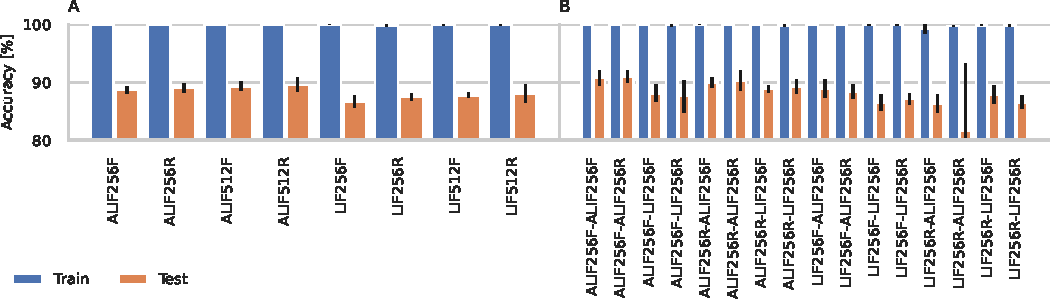
\includegraphics{figures/dense_accuracy.pdf}
  \caption{Accuracy on the testing and training set of the DVS gesture dataset~\citep{amir_low_2017} on one (A) and two (B) layer classifiers trained with e-prop~\citep{Bellec2020}.
  All models were trained for 100 epochs with a batch size of 512.
  Bars signify the mean and error bars the standard deviation of 5 models trained with different seeds.}
  \label{fig:dense_accuracy}
\end{figure*}

\subsection{Using models for training and inference}
Once a network structure has been defined, mlGeNN provides a range of \emph{compilers} to produce GeNN models which can then be used for training or inference.
The simplest compiler is the \lstinline{InferenceCompiler} which builds a GeNN model with static weights and parallel batching support for efficiently performing inference on an SNN model:
\begin{lstlisting}[language=Python]
compiler = InferenceCompiler(
    evaluate_timesteps=1500, batch_size=512)

compiled_net = compiler.compile(network)
\end{lstlisting}
The resulting \lstinline{compiled_net} object can then be used to evaluate the network on a dataset:
\begin{lstlisting}[language=Python]
metrics, _  = compiled_net.evaluate(
    {input: inputs}, {output: labels})
\end{lstlisting}
By default, the evaluation method calculates sparse categorical accuracy against the provided labels but mlGeNN also provides alternative metrics for regression tasks and custom metrics can easily be implemented.
As well as supporting the conversion of trained ANN models to SNNs as described in our previous work~\citep{Turner2022}, mlGeNN now provides an e-prop compiler which can be used to train models with the e-prop learning rule~\citep{Bellec2020}.
This compiler checks the validity of the model and automatically adds the appropriate learning rules to its connections as well as feedback connections and error signal calculation logic:
\begin{lstlisting}[language=Python]
compiler = EPropCompiler(
    example_timesteps=1500,
    losses="sparse_categorical_crossentropy",
    optimiser="adam", batch_size=512)

compiled_net = compiler.compile(network)
\end{lstlisting}
Note that here again, loss functions and optimisers with default parameters are specified using strings but these are also fully customisable.
After compiling with the \lstinline{EPropCompiler}, the \lstinline{compiled_net} object can then be used to train the network on a dataset:

\begin{lstlisting}[language=Python]
metrics, _  = compiled_net.train(
    {input: inputs}, {output: labels},
    num_epochs=args.num_epochs, shuffle=True)
\end{lstlisting}

\begin{figure*}[t]
  \centering
  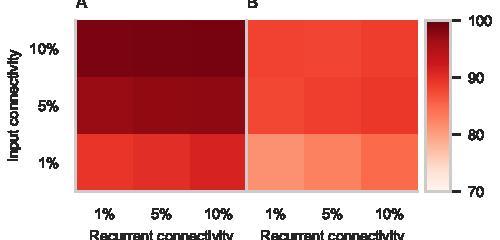
\includegraphics{figures/sparse_accuracy.pdf}
  \caption{Accuracy on the testing and training set of the DVS gesture dataset~\citep{amir_low_2017} on sparse models with (A) ALIF512R (B) ALIF256F-ALIF256R architectures and varying levels of sparsity trained with e-prop~\citep{Bellec2020}.
  All models were trained for 100 epochs with a batch size of 512.
  Sparsity measure describes the fixed probability of there being a synapse between any two neurons (with no self connections in the recurrent connectivity).
  Bars signify the mean and error bars the standard deviation of 5 models trained with different seeds.}
  \label{fig:sparse_accuracy}
\end{figure*}

\subsection{Recording and debugging}
One of the challenges of working with SNNs, compared to standard ANNs, is that neurons are stateful so the ability to efficiently record and visualise model state is vital for an efficient workflow.
Inspired by Keras, mlGeNN has a callback system which -- as well as being used internally to implement progress bars, trigger processes such as weight updates during model training etc -- can be used by the user to configure the recording of state variables and spikes.

\lstinline{VarRecorder} can be used to record a population state variable over time and \lstinline{SpikeRecorder} can be used to efficiently record spikes (using the efficient system described in \citet{Knight2021}).
For example here, we record the spikes emitted by the first layer \lstinline{a} and the membrane voltages of the second  layer \lstinline{b} of the previous example:
\begin{lstlisting}[language=Python]
callbacks = [SpikeRecorder(a, key="a_spikes"),
             VarRecorder(b, "V", key="b_v")]
metrics, cb_data = compiled_net.evaluate(
    {input: inputs}, {output: labels},
    callbacks=callbacks)
\end{lstlisting}
The \lstinline{key} strings are used to uniquely identify recorded data produced by callbacks and, after the simulation has completed, allow the user to retrieve the recorded variables from the \lstinline{cb_data} dictionary which is returned when evaluating (or training) the model.
For example, the membrane voltages emitted by all neurons during the presentation of the first input pattern could be accessed using \lstinline{cb_data["b_v"][0]}.

In machine learning workflows, where models may be trained for millions of timesteps, it is also important to be able to \emph{filter} what data is recorded to particular areas/stages of training to save memory and reduce overheads.
Both \lstinline{SpikeRecorder} and \lstinline{VarRecorder} support filtering by neuron or example, e.g. \\ \lstinline{SpikeRecorder(a, neuron=np.s_[0::2])} could be used to record spikes from every other neuron and \lstinline{SpikeRecorder(a, example_filter=1000)} could be used to only record during the 1000th example.

\section{Results}
In order to demonstrate the value of mlGeNN for spike-based ML research, we here present the results of a small exploration of SNN architectures, trained using e-prop~\citep{Bellec2020} on the DVS gesture dataset~\citep{amir_low_2017}, which has recently been used to evaluate the EGRU~\citep{subramoney2022egru} and FPTT~\citep{yin2021accurate} learning rules.
This dataset consists of \num{1342} recordings of \num{11} different hand and arm gestures, collected from \num{29} subjects under three different lighting condition using a DVS 128 event-based camera~\citep{lichtsteiner_128times128_2008}.
We used the Tonic library~\citep{lenz_gregor_2021_5079802} to access the dataset and spatially downsample the events to $32\times32$.
While mlGeNN does not depend on Tonic, it includes a \lstinline{preprocess_tonic_spikes} helper function which converts spike trains from Tonic datasets into mlGeNN's internal format.

\subsection{Accuracy}
Figure~\ref{fig:dense_accuracy} shows the accuracy of a wide selection of one and two layer classifier models trained with e-prop.
These include configurations with and without recurrent connections and using both Adaptive and standard Leaky Integrate-and-Fire~(ALIF and LIF) neuron models.
Of the single layer classifiers, the variant with a single layer of 512 recurrently connected ALIF neurons performs the best, achieving an accuracy of \SI{89.55 \pm 1.22}{\percent} on the test set.
Although this model only has a single hidden layer and around \num{1.3E6} parameters, it out-performs a two layer EGRU model~\citep{subramoney2022egru} with over $4\times$ as many parameters which achieved \SI{88.02}{\percent} accuracy.

Models using ALIF neurons also perform better than those using simpler LIF neurons in all of the two layer configurations.
Interestingly, similar to the architecture employed by \citet{yin2021accurate}, the best performing model -- with an accuracy of \SI{91.00 \pm 1}{\percent} on the test set -- has a feedforward first layer followed by a recurrent second layer rather than two recurrently connected layers.
While this performance is slightly lower than the \SI{91.89 \pm 0.16}{\percent} reported by \citet{yin2021accurate}, our model has approximately a third the number of parameters (\num{0.66e6} vs \num{1.8e6}).

One of the significant advantages of mlGeNN is that it can exploit sparse connectivity to reduce training and inference time so, in the final part of our architectural exploration, we explore the effect of sparsity on the performance of our two best performing models (ALIF512R and ALIF256F-ALIF256R).
The results of this exploration are shown in figure~\ref{fig:sparse_accuracy} and, while increasing sparsity clearly impacts performance, sparse configurations of ALIF512R are still highly competitive.
In fact, the best oerforming ALIF512R configuration -- with \SI{5}{\percent} connectivity in the input connections and \SI{10}{\percent} connectivity in the recurrent connections -- still out-performs the two layer EGRU model~\citep{subramoney2022egru}, even though it only has over $60\times$ fewer parameters.

\begin{figure}[t]
  \centering
  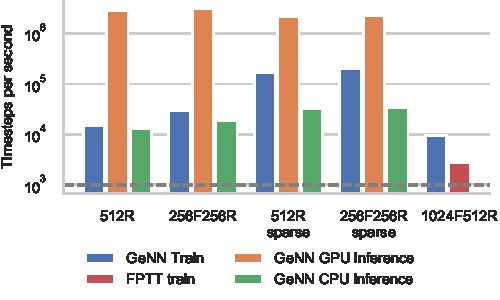
\includegraphics{figures/performance.pdf}
  \caption{Throughput of inference and training best two models on the DVS gesture dataset~\citep{amir_low_2017}.
  GPU training was performed with a batch size of 512 and inference with a batch size of 264 (the full size of the test set).}
  \label{fig:performance}
\end{figure}

\subsection{Performance}
\begin{itemize}
    \item Training time - compare to FPTT \SI{400}{\milli\second} per frame with batch size 64 on some sort of \SI{24}{\giga\byte} GPU
    \item Inference time CPU and GPU - compare to real-time
    \item Show effect of sparsity on performance
\end{itemize}

\section{Conclusions}
We hope that the mlGeNN library described in this paper will be as valuable to the community as it was in generating the results presented here.
While it is by no means a precise measure, the simplicity and ease of
using mlGeNN is illustrated by the fact that the code used for all
simulations presented here was less than \num{300} lines whereas, when we used PyGeNN directly in our previous work~\citep{Knight2022} one \num{900} line model was required for training and a seperate \num{500} line model for inference.

The e-prop learning rule is an approximation to gradient descent, both in terms of using a surrogate gradient and in neglecting some terms relating to recurrent connections.
The results we have presented in this paper demonstrate that this approximate nature of the e-prop learning rule does not necessarily prevent it from offering competitive performance on relatively complex datasets.
However, e-prop has properties that could be seen as disadvantageous for fast and efficient learning and inference.
Firstly, e-prop requires time-driven updates of synaptic variables which dominates the time taken to train models.
We demonstrate that by using sparse connectivity, this problem can be reduced and, in initial unpublished experiments, we have found that by combining sparse connectivity with the Deep-R~\citep{Bellec2018a} rewiring rule, much of the performance lost due to the sparser connectivity can be recovered.
Secondly and unsuprisingly for a visual task, both the original experiments on the DVS gesture dataset~\citep{amir_low_2017} and more recent work using the Decolle and FPTT learning rules~\citep{Kaiser2020,yin2021accurate}, showed that a convolutional SNN can achieve significantly higher performance than shallow recurrent networks.
However, because the eligibility traces which drive e-prop weight updates are calculated from the product of pre and postsynaptic activity, they cannot be shared across the corresponding synapses in a convolutional layer.
Each synapse needs individual state variabes.
Neither the FPPT~\citep{yin2021accurate} learning rule -- where the additional $\bar{\Phi}_t$ state variable only depends on past weights so can be shared -- nor EventProp~\citep{Wunderlich2021} -- which does not require any additional synaptic state -- have these issues so are much more suitable for training convolutional architectures.

Therefore, based on the promising initial results presented by \citet{NowotnyLoss2022}, we are working to develop an mlGeNN compiler for the EventProp~\citep{Wunderlich2021} learning rule which will allow convolutional models to be trained and to reduce training times by taking advantage of temporal sparsity through purely event-driven training.
%%
%% The acknowledgments section is defined using the "acks" environment
%% (and NOT an unnumbered section). This ensures the proper
%% identification of the section in the article metadata, and the
%% consistent spelling of the heading.
\begin{acks}
This work was funded by the EPSRC (grant numbers EP/V052241/1 and EP/S030964/1) and the EU's Horizon 2020 program (grant agreement 945539).
Compute time was provided through Gauss Centre for Supercomputing application number 21018 and EPSRC (grant number EP/T022205/1) and local GPU hardware was provided by an NVIDIA hardware grant award.
\end{acks}

%%
%% The next two lines define the bibliography style to be used, and
%% the bibliography file.
\balance
\bibliographystyle{ACM-Reference-Format}
\bibliography{ml_genn_eprop}

\end{document}
\endinput
%%
%% End of file `sample-sigconf.tex'.
